\newpage
\appendix

% \section{Proof}
% % 學到的結果會是機率連乘
% We show that for any state $s_t$ and its dominant option $o_{t+1} = \{a_{t+1}, a_{t+2}, ..., a_{t+l}\}$ with length $0\leq l\leq L$, the training target $\Phi_t = \{\phi_t,\phi_{t+1},...,\phi_{t+L-1}\}$ designed according to the composite actions $\mathcal{O}_1, \mathcal{O}_2, ...$ enables the option network to learn the cumulative probability $P(o_{t+1})=\prod_{i=1}^l P(a_{t+i})$.

% $\omega^k_l(a^*_{t_k+l})=P(a^*_{t_k+2},a^*_{t_k+3},...,a^*_{t_k+l}|s_{t_k},a^*_{t_k+1})$.
% The action used in the environment $a_{t_k+1}$ is sampled from the MCTS search policy $\pi_{t_k}$.
% The label is divided into three cases:
% \begin{enumerate}
%     \item $a_{t_k+1}\neq a^*_{t_k+1}$: with probability $1-\pi_{t_k}(a^*_{t_k+1})$, no loss is applied to $\omega^k_l(a^*_{t_k+l})$
%     \item $a_{t_k+1}=a^*_{t_k+1}$ and $\forall 1<i<l, a_{t_k+i}=a^*_{t_k+i}$: with probability $\prod_{i=0}^{l-2} \pi_{t_k+i}(a^*_{t_k+i+1})$, it learns $\omega^k_l(a^*_{t_k+l})=\pi_{t_k+l-1}$
%     \item $a_{t_k+1}=a^*_{t_k+1}$ but $\exists 1<i\leq l, a_{t_k+i}\neq a^*_{t_k+i}$: with probability $\pi_{t_k}(a^*_{t_k+1})-\prod_{i=0}^{l-2} \pi_{t_k+i}(a^*_{t_k+i+1})$, it learns $\omega^k_l(a^*_{t_k+l})=0$
% \end{enumerate}
% Since in the first case there is no loss applied to $\omega^k_l(a^*_{t_k+l})$, averaging the results of the last two cases we get:
% \begin{equation}
%     \begin{split}
%         \omega^k_l(a^*_{t_k+l})&=\frac{(\prod_{i=0}^{l-2} \pi_{t_k+i}(a^*_{t_k+i+1}))*\pi_{t_k+l-1}(a^*_{t_k+l})+(\pi_{t_k}(a^*_{t_k+1})-\prod_{i=0}^{l-2} \pi_{t_k+i}(a^*_{t_k+i+1}))*0}{\pi_{t_k}(a^*_{t_k+1})}\\
%         &=\prod_{i=1}^{l-1} \pi_{t_k+i}(a^*_{t_k+i+1})\\
%         &=P(a^*_{t_k+2},a^*_{t_k+3},...,a^*_{t_k+l}|s_{t_k},a^*_{t_k+1})
%     \end{split}
% \end{equation}

% 如果有兩個以上的max,則會學成stop
% For the designed label, if the max action at time-step $t_k+l$ is not unique, $\argmax_a \omega^k_l(a)=stop$.
% Assume at time-step $t_k+l$, there are $N$ actions, and $M$ actions are max actions with probability $\pi_{t_k+l}(a^*_{t_k+l+1}))=x$.
% The $M$ max actions learn probability:
% \begin{equation}
%     \begin{split}
%         \omega^k_l(a^*_{t_k+l})&=\frac{(\prod_{i=0}^{l-2} \pi_{t_k+i}(a^*_{t_k+i+1}))*\pi_{t_k+l-1}(a^*_{t_k+l})+(M*\pi_{t_k}(a^*_{t_k+1})-\prod_{i=0}^{l-2} \pi_{t_k+i}(a^*_{t_k+i+1}))*0}{M*\pi_{t_k}(a^*_{t_k+1})}\\
%         &=\frac{\prod_{i=1}^{l-1} \pi_{t_k+i}(a^*_{t_k+i+1})}{M}
%     \end{split}
% \end{equation}
% The stop learns probability:
% \begin{equation}
%         \omega^k_l(stop)=1-M*\omega^k_l(a^*_{t_k+l})=1-\prod_{i=1}^{l-1} \pi_{t_k+i}(a^*_{t_k+i+1})\\
% \end{equation}
% Since probability distribution sums up to 1, and each element in the distribution is less than or equal to 1, we have:
% \begin{equation}
%         \omega^k_l(a^*_{t_k+l})=\frac{\prod_{i=1}^{l-1} \pi_{t_k+i}(a^*_{t_k+i+1})}{M}\leq \frac{\pi_{t_k+l-1}(a^*_{t_k+l})}{M} \leq \frac{\frac{1}{M}}{M} = \frac{1}{M^2}
% \end{equation}
% \begin{equation}
%         \omega^k_l(stop)=1-M*\omega^k_l(a^*_{t_k+l})\geq 1-M*\frac{1}{M^2}=1-\frac{1}{M}\\
% \end{equation}
% When $M>=2$,
% \begin{equation}
%         \omega^k_l(stop)\geq 1-\frac{1}{M}> \frac{1}{M^2}\geq \omega^k_l(a^*_{t_k+l})\\
% \end{equation}
% Therefore, $\argmax_a \omega^k_l(a)=stop$ when the max action at time-step $t_k+l$ is not unique.

\clearpage


\section{Implementation details}
\label{appendix:implementation}

In this section, we detail our OptionZero implementation, which is built upon a publicly available MuZero framework \cite{wu_minizero_2024}.

\subsection{MCTS details}

The MCTS implementation mainly follows that introduced in Section \ref{sec:ozero-mcts}, with minor details described below.

\paragraph{Dirichlet noise}
To encourage exploration, in MuZero, Dirichlet noise is applied to the root node.
Similarly, in OptionZero, since option can also be executed in the environment, we apply Dirichlet noise to both primitive selection and option selection at the root node.

\paragraph{Default estimated Q value}
For primitive selection, we follow the default estimated Q value for Atari games in the framework \cite{wu_minizero_2024} that enhances exploration:
\begin{equation}
\hat{Q}(s) = 
\begin{cases}
\frac{Q_{\Sigma}(s)}{N_{\Sigma}(s)} & N_{\Sigma}(s)>0\\
1 & N_{\Sigma}(s)=0,
\end{cases} \\
\end{equation}
where $N_{\Sigma}(s) = \sum_{b} \mathbf{1}_{N(s,b)>0}$, $Q_{\Sigma}(s) = \sum_{b} \mathbf{1}_{N(s,b)>0}Q(s,b)$, and $\mathbf{1}_{N(s,b)>0}$ is the characteristic function that only considers primitive child nodes with non-zero visit counts.

For option selection, since the contributions of option child node are included in the statistics of its corresponding predecessor primitive child node, we use a default estimated Q value that incorporates a virtually losing outcome:
\begin{equation}
\hat{Q}(s) = \frac{Q_(s,a)\times N(s,a)}{N(s,a)+1},
\end{equation}
where $N(s,a)$ is the visit counts of the primitive child node, and $Q_(s,a)$ is the mean value of the primitive child node.

% \paragraph{Calculation of estimated Q value}
% In backup, the discounted reward from the root node to a node $s^i$ is available only if $s^i$ is evaluated, while there may be some nodes $s^j$ that are unevaluated due to it may skipped by option .
% In practice, the estimated Q value is only required at evaluated nodes in selection, since as an unevaluated node is reached, the selection phase is done.
% As a result, we split the derivation of Q value at node $s^i$ into two parts.
% First, in backup, the $l$-step estimate of cumulative discounted reward from $s^l$ to $s^0$ is updated to all edges on the possible path from $s^0$ to $s^l$.
% Then, when a node $s^i$ is evaluated 
% MCTS detail
% option initQ
% option dirichlet noise
% backup
% only need to do selection at evaluated node
% If node $s^k$ is not evaluated, we can not compute $G_{k,i}$ since $r_{0,k}$ is not available by previous selection paths, so we temporally update the mean value of primitive edges by $Q(s^k,a)=\frac{(N(s^{k+1})-1)\cdot Q(s^k,a)+G_{0,i}}{N(s^{k+1})}$, the mean value of option edge by $Q(s^k,O^k)=\frac{(N(s^{k+L})-1)\cdot Q(s^k,O^k)+G_{0,i}}{N(s^{k+L})}$ and correct the value when the node is expanded.
% The value is corrected by $Q(s^k,a)=\frac{Q(s^k,a)-r_{0,k}}{\gamma^k}$ and $Q(s^k,O^k)=\frac{Q(s^k,O^k)-r_{0,k}}{\gamma^k}$, respectively.

% \paragraph{\revision{Option statistics}}
% \revision{
% In practice, an efficient approach is to store the statistics on the node and use them to derive edge statistics ($N$, $R$, and $Q$), eliminating the additional cost of traversing all possible edges during backup.
% Here, we take the search tree in Figure \ref{fig:search-tree-implementation-example} as an example to illustrate the approach.
% To make it easier to distinguish the edge statistics and node statistics, we use a different notation of statistics in this example: $\bar{N}_{i,j}$, $\bar{R}_{i,j}$, and $\bar{Q}_{i,j}$ represent the visit count, reward, and Q value of an edge from node $i$ to node $j$; $\dot{N}_i$, $\dot{R}_i$, and $\dot{Q}_i$ represent the node statistics of node $i$.
% First, for the visit count $\bar{N}_{i,j}$, we simply store it as $\dot{N}_j$ since the visit counts of multiple edges to the same target node should all be the same for consistency, e.g., $\bar{N}_{a,c} = \bar{N}_{b,c} = \dot{N}_c$.
% Second, for the reward $\bar{R}_{i,j}$, we store the cumulative reward from the root node to $j$ as $\dot{R}_j$, and calculate the edge reward by $\bar{R}_{i,j} = \dot{R}_j - \dot{R}_i$.
% Third, for the Q value $\bar{Q}_{i,j}$ of each edge, we maintain the Q value $\dot{Q}_j$ of each node instead, which is defined in a similar way as the edge -- the sum of the cumulative reward and the node value.
% Thus, it can be derived that $\bar{Q}_{i,j} = \dot{Q}_j - \dot{R}_i$.
% Note that we omit the discount factor in this example for easier understanding; it should be introduced for rewards and Q values using the method discussed in Section \ref{sec:ozero-mcts} (Backup) in practice.
% }
% \begin{figure}[h]
%     \centering
%     \includegraphics[width=0.15\linewidth]{figures/mcts_example_implementation.pdf}
%     \caption{\revision{An example search tree with an option.}}
%     \label{fig:search-tree-implementation-example}
% \end{figure}

\subsection{\revision{MCTS complexity}}
\revision{
% Note that in OptionZero, the complexity of MCTS remains the same as the original. In the selection phase, the only added step is comparing the PUCT scores of option child nodes and primitive child nodes. In the expansion phase, while more nodes are initially expanded, each simulation still evaluates only one node at a time. The backup phase does not introduce additional complexity since the statistical information for option edges can be derived from primitive edges. As a result, only the statistics for primitive edges need to be stored and updated. The main additional cost lies in introducing a new head to predict the dominant option, but since most weights in the option network are shared with the rest of the network, the impact on runtime is small.
The complexity of the modified MCTS remains the same as the original, with additional minor computational costs in introducing a new network head to predict and use the dominant option.
Specifically, in the selection phase, the only added step is comparing the PUCT scores of option child nodes and primitive child nodes, as in \eqref{eq:option_mcts_puct}.
In the expansion phase, the option policy $\Omega$ is evaluated along with policy $p$ and value $v$.
Since most network weights of the option policy head are shared with the rest of the network, the impact on runtime is negligible. 
While more nodes are initially expanded, each simulation evaluates only one node at a time. 
% In the backup phase, there is no additional cost since only the statistics for primitive edges need to be stored and updated, as in \eqref{eq:option_mcts_backup}.
% Note that the statistical information for option edges can be derived from primitive edges, so they do not need to be stored.
In the backup phase, as the statistics of option edges can be easily derived from primitive edges, only the statistics of primitive edges are maintained in practice, eliminating the additional cost of updating all possible option edges.
}

\subsection{GridWorld environment}
The implementation is also built upon the same framework \cite{wu_minizero_2024}, with a custom GridWorld environment added.
The reward of the environment is defined as follows: the initial total reward is 200 points, and for each action or option taken, one point is deducted from the reward.

\subsection{Network architecture}
The network architecture follows a structure similar to MuZero.
As discussed in Section \ref{sec:ozero}, the option network is incorporated into the prediction network.
% by adding additional fully connected layers in the policy head for option prediction, which are initialized to predict $stop$ for each head.
Specifically, besides the policy head, we add additional $L-1$ option heads for predicting $\Omega=\{\omega_2,\omega_3,...,\omega_L\}$, initialized to predict the $stop$.
Note that there is no need for extra prediction of $\omega_1$, since we can directly get the first action of the dominant option from policy head by choosing $a^*_1=\argmax_a p(a)$.
Additionally, the dynamics network is modified to simulate the environment transitions of executing both primitive actions and options.
By extending the original action input, the action sequence input to the dynamics network is encoded into a fixed number of $L$ planes for supporting options with different lengths, with the $l$th plane corresponding to the $l$th move inside an option.
Note that when $l<L$, the subsequent planes are set to zero, representing no moves.
% The first $l$ planes encode one corresponding action per plane, while the remaining planes are set to zero, where $l$ represents the length of the action sequence, and $1\leq l\leq L$.

\paragraph{Atari games}
We additionally adopt the state consistency \cite{ye_mastering_2021}.
Therefore, the SimSiam \cite{chen_exploring_2021} architecture is included to calculate the consistency loss.

\paragraph{GridWorld}
The network architecture generally follows the architecture tailored for Atari games.
However, in the design of the representation network, we removed the down-sampling mechanism, adopting a setup similar to MuZero for board games as in \citet{wu_minizero_2024}.
% is essentially the same as the one used for Atari games.
% However, we set the number of blocks to one, and in the design of the representation network, we removed the down-sampling mechanism used for Atari games, adopting a setup similar to MuZero for board games as in \citet{wu_minizero_2024}.

\section{Training OptionZero}
\label{appendix:experiment-setup}

In this section, we describe the details for training OptionZero models used in the experiments.
The experiments are conducted on machines with 24 CPU cores and four NVIDIA GTX 1080 Ti GPUs.
For the training configurations, we generally follow those in MuZero, where the hyperparameters are listed in Table \ref{tab:hyperparameters}.

\section{Hyperparameter Search}\label{app:hype}
\normalsize
We exclusively conduct hyperparameter search on fold 0. 
For \textbf{GraFITi}~\citep{Yalavarthi2024.GraFITi} the hyperparameters for the search are as follows:
\begin{itemize}
    \item The number of layers, with possible values [1, 2, 3, 4].
    \item The number of attention heads, with possible values [1, 2, 4].
    \item The latent dimension, with possible values [16, 32, 64, 128, 256].
\end{itemize}

For the \textbf{LinODEnet} model~\citep{Scholz2022.Latenta} we search the hyperparameters from:
\begin{itemize}
    \item The hidden dimension, with possible values [16, 32, 64, 128].
    \item The latent dimension, with possible values [64, 128, 192, 256].
\end{itemize}

For \textbf{GRU-ODE-Bayes}~\citep{DeBrouwer2019.GRUODEBayesd} we tune the hidden size from [16, 32, 64, 128, 256]

For \textbf{Neural Flows}~\citep{Bilos2021.Neurald} we define the hyperparameter spaces for the search are as follows:
\begin{itemize}
    \item The number of flow layers, with possible values [1, 2, 4].
    \item The hidden dimension, with possible values [16, 32, 64, 128, 256].
    \item The flow model type, with possible values [GRU, ResNet].
\end{itemize}

For the \textbf{CRU}~\citep{Schirmer2022.Modelingb} the hyperparameter space is as follows:
\begin{itemize}
    \item The latent state dimension, with possible values [10, 20, 30].
    \item The number of basis functions, with possible values [10, 20].
    \item The bandwidth with possible values [3, 10].
\end{itemize}

% rebuttal TODO
% 時間
\paragraph{Atari games}
For Atari games, each setting is trained for 3 runs on each game, with each model taking approximately 22 hours to complete.
\revision{
Since we introduce an additional head to predict option, the training time slightly increases as the max option length increases.
For $\ell_1$, the training time is approximately 21.89 hours.
For $\ell_3$ and $\ell_6$, the training times increase to around 22.28 hours and 22.95 hours, representing increases of 1.8\% and 4.8\%, respectively.
}
The performance is measured based on the average score of the latest 100 completed games in each run during the training \cite{hessel_muesli_2021}.
The training curves are shown in Figure \ref{fig:atari26}.

\begin{figure*}[h!t]
\centering
% \vspace*{-10em}
\subfloat{
    \includegraphics[width=0.25\linewidth]{figures/atari26/alien.pdf}}
\subfloat{
    \includegraphics[width=0.25\linewidth]{figures/atari26/amidar.pdf}}
\subfloat{
    \includegraphics[width=0.25\linewidth]{figures/atari26/assault.pdf}}
\subfloat{
    \includegraphics[width=0.25\linewidth]{figures/atari26/asterix.pdf}}
\\\vspace*{0em}
\subfloat{
    \includegraphics[width=0.25\linewidth]{figures/atari26/bank_heist.pdf}}
\subfloat{
    \includegraphics[width=0.25\linewidth]{figures/atari26/battle_zone.pdf}}
\subfloat{
    \includegraphics[width=0.25\linewidth]{figures/atari26/boxing.pdf}}
\subfloat{
    \includegraphics[width=0.25\linewidth]{figures/atari26/breakout.pdf}}
\\\vspace*{0em}
\subfloat{
    \includegraphics[width=0.25\linewidth]{figures/atari26/chopper_command.pdf}}
\subfloat{
    \includegraphics[width=0.25\linewidth]{figures/atari26/crazy_climber.pdf}}
\subfloat{
    \includegraphics[width=0.25\linewidth]{figures/atari26/demon_attack.pdf}}
\subfloat{
    \includegraphics[width=0.25\linewidth]{figures/atari26/freeway.pdf}}
\\\vspace*{0em}
\subfloat{
    \includegraphics[width=0.25\linewidth]{figures/atari26/frostbite.pdf}}
\subfloat{
    \includegraphics[width=0.25\linewidth]{figures/atari26/gopher.pdf}}
\subfloat{
    \includegraphics[width=0.25\linewidth]{figures/atari26/hero.pdf}}
\subfloat{
    \includegraphics[width=0.25\linewidth]{figures/atari26/jamesbond.pdf}}
\\\vspace*{0em}
\subfloat{
    \includegraphics[width=0.25\linewidth]{figures/atari26/kangaroo.pdf}}
\subfloat{
    \includegraphics[width=0.25\linewidth]{figures/atari26/krull.pdf}}
\subfloat{
    \includegraphics[width=0.25\linewidth]{figures/atari26/kung_fu_master.pdf}}
\subfloat{
    \includegraphics[width=0.25\linewidth]{figures/atari26/ms_pacman.pdf}}
\\\vspace*{0em}
\subfloat{
    \includegraphics[width=0.25\linewidth]{figures/atari26/pong.pdf}}
\subfloat{
    \includegraphics[width=0.25\linewidth]{figures/atari26/private_eye.pdf}}
\subfloat{
    \includegraphics[width=0.25\linewidth]{figures/atari26/qbert.pdf}}
\subfloat{
    \includegraphics[width=0.25\linewidth]{figures/atari26/road_runner.pdf}}
\\\vspace*{0em}
\subfloat{
    \includegraphics[width=0.25\linewidth]{figures/atari26/seaquest.pdf}}
\subfloat{
    \includegraphics[width=0.25\linewidth]{figures/atari26/up_n_down.pdf}}
\subfloat{
    \includegraphics[width=0.25\linewidth]{figures/atari26/label.pdf}}
\caption{Training curves on 26 Atari games.}
\label{fig:atari26}
\end{figure*}



\paragraph{GridWorld}
In this toy example, we aim to clearly show that the length of the learned options can be extended as the training time increases.
For training, we use a maximum option length $L = 9$, fixing the goal position and selecting random starting points.
As for the evaluation, we fix the starting point and the goal as shown in Figure \ref{fig:maze}.
The evaluation also uses 50 MCTS simulations, and the original softmax function is replaced with max selection.

\clearpage

\section{Ablation study for OptionZero}

For the ablation study, we train OptionZero with a maximum option length $L = 3$, but disable the execution of options in the environment, using them solely for MCTS planning, denoted as n-$\ell_3$.
Since all composite actions are primitive actions, we define each $o_i$ as $\{a_{i+1}\}$, where $a_{i+1}=\argmax_a p_i(a)$ and train the option network according to the policy network.
According to the results shown in Table \ref{tab:Atari26-ablation}, n-$\ell_3$ achieves a mean human-normalized score of 1008.15\%, which is 85.43\% higher than the baseline $\ell_1$, indicating that OptionZero still enhances MCTS planning with options without executing them.
Notably, in games that require precise step-by-step predictions, such as \textit{gopher}, n-$\ell_3$ outperforms $\ell_3$, indicating that planning for every step remains crucial for certain games.
However, in games that benefit from bypassing unimportant frames, such as \textit{seaquest}, the performance of n-$\ell_3$ is only comparable to baseline.

\begin{table*}[h!t]
    \centering
    \caption{Scores on 26 Atari games for the ablation study. Bold text in $\ell_3$ and n-$\ell_3$ indicates scores that surpass $\ell_1$.}
    \resizebox{0.85\textwidth}{!}{
    \begin{tabular}{l|rr|rrrrr}
    \toprule
        \multirow{3}{*}{Game} & \multirow{3}{*}{Random} & \multirow{3}{*}{Human} && \multicolumn{3}{c}{OptionZero} \\
        \cline{5-7}
        & & & & \makecell[c]{$\ell_1$} & \makecell[c]{$\ell_3$} & \makecell[c]{n-$\ell_3$} \\
    \midrule
alien & 128.30 & 6,371.30 &&  2,437.30  & \textbf{2,900.07} & \textbf{3,523.20} \\
amidar & 11.79 & 1,540.43 &&  780.26  & \textbf{820.77} & \textbf{848.97} \\
assault & 166.95 & 628.89 &&  18,389.88  & \textbf{19,302.04} & \textbf{19,378.79} \\
asterix & 164.50 & 7,536.00 &&  177,128.50  & \textbf{188,999.00} & \textbf{202,183.33} \\
bank heist & 21.70 & 644.50 &&  1,097.63  &  950.13  &  1,081.10  \\
battle zone & 3,560.00 & 33,030.00 &&  53,326.67  & \textbf{53,583.33} & \textbf{65,660.00} \\
boxing & -1.46 & 9.61 &&  97.71  &  95.09  &  94.58  \\
breakout & 1.77 & 27.86 &&  371.30  & \textbf{375.58} & \textbf{427.18} \\
chopper command & 644.00 & 8,930.00 &&  43,951.67  & \textbf{60,181.67} & \textbf{79,340.33} \\
crazy climber & 9,337.00 & 32,667.00 &&  110,634.00  & \textbf{114,390.00} & \textbf{122,865.67} \\
demon attack & 208.25 & 3,442.85 &&  103,823.17  & \textbf{117,270.57} & \textbf{104,351.00} \\
freeway & 0.17 & 25.61 &&  29.46  & \textbf{31.06} & \textbf{30.93} \\
frostbite & 90.80 & 4,202.80 &&  3,183.40  & \textbf{3,641.10} & \textbf{3,923.63} \\
gopher & 250.00 & 2,311.00 &&  70,985.27  &  68,240.60  & \textbf{73,338.67} \\
hero & 1,580.30 & 25,839.40 &&  13,568.20  & \textbf{19,073.18} & \textbf{14,181.65} \\
jamesbond & 33.50 & 368.50 &&  8,155.50  & \textbf{13,276.67} &  7,172.17  \\
kangaroo & 100.00 & 2,739.00 &&  8,929.67  & \textbf{12,294.00} & \textbf{11,175.33} \\
krull & 1,151.90 & 2,109.10 &&  10,255.37  &  10,098.83  & \textbf{17,420.13} \\
kung fu master & 304.00 & 20,786.80 &&  66,304.67  & \textbf{68,528.33} & \textbf{67,735.67} \\
ms pacman & 197.80 & 15,375.05 &&  3,695.60  & \textbf{4,952.37} & \textbf{4,762.23} \\
pong & -17.95 & 15.46 &&  19.37  &  15.49  & \textbf{20.01} \\
private eye & 662.78 & 64,169.07 &&  116.83  &  90.76  &  94.71  \\
qbert & 159.38 & 12,085.00 &&  17,155.50  & \textbf{30,748.42} & \textbf{22,321.75} \\
road runner & 200.00 & 6,878.00 &&  26,971.33  & \textbf{32,786.67} &  23,784.67  \\
seaquest & 215.50 & 40,425.80 &&  3,592.53  & \textbf{5,606.63} &  3,378.60  \\
up n down & 707.20 & 9,896.10 &&  217,021.60  & \textbf{280,832.43} & \textbf{238,409.40} \\
\midrule                 
Normalized Mean & 0.00 & 100.00 \% &&  922.72 \%  & \textbf{1054.30 \%} & \textbf{1008.15 \%} \\
Normalized Median & 0.00 & 100.00 \% &&  328.40 \%  & \textbf{391.69 \%} & \textbf{341.19 \%} \\
    \bottomrule
    \end{tabular}
}
    \label{tab:Atari26-ablation}
\end{table*}


\clearpage

\section{In-depth behavior analysis}\label{appendix:behavior-analysis}

In this experiment section, we conduct detailed analysis for $\ell_3$ and $\ell_6$ in 26 Atari games.

\subsection{Options applied in games}
\label{appendix:options-applied}

We present the statistics in all 26 Atari games conducted for the behavior analysis in Section \ref{sec:behavior-analysis}.
Specifically, we provide the numbers of options types, option usages, proportions of options with repeated actions, and the average option lengths for $\ell_3$ and $\ell_6$ in Table \ref{tab:option-usage-op3} and Table \ref{tab:option-usage-op6}, respectively.
The columns ``\# \{$a$\}'' and ``\# \{$o$\}'' show the numbers of available primitive actions and the numbers of the options recorded during evaluation, columns ``\% $a$'' and ``\% $o$'' show the proportions of actions and options applied during the game, columns ``\% Rpt.'' and ``\% NRpt.'' show the proportions of options with repeated primitive actions and options with more than one action type, and column ``$\bar{l}$'' shows the average options length (including primitive action).
We also provide the proportions of options with different lengths for both  $\ell_3$ and $\ell_6$ in Table \ref{tab:option-length-op3-op6}.

\begin{table}[h!]
\caption{Numbers of option types, option usages, proportions of options with repeated actions, and average option lengths for $\ell_3$ in 26 Atari games.}
\centering
\small
\begin{tabular}{l|rrrrrrr}
    \toprule
    Game & \# \{$a$\} & \# \{$o$\} & \% $a$ & \% $o$ & \% Rpt. & \% NRpt. & $\bar{l}$ \\
    \midrule
    alien & 18 & 185 & 67.66\% & 32.34\% & 94.54\% & 5.46\% & 1.61 \\
    amidar & 10 & 187 & 65.51\% & 34.49\% & 98.43\% & 1.57\% & 1.65 \\
    assault & 7 & 139 & 78.84\% & 21.16\% & 57.20\% & 42.80\% & 1.30 \\
    asterix & 9 & 163 & 92.82\% & 7.18\% & 90.74\% & 9.26\% & 1.10 \\
    bank heist & 18 & 138 & 41.93\% & 58.07\% & 7.60\% & 92.40\% & 2.05 \\
    battle zone & 18 & 217 & 88.89\% & 11.11\% & 95.33\% & 4.67\% & 1.18 \\
    boxing & 18 & 240 & 39.53\% & 60.47\% & 50.54\% & 49.46\% & 2.12 \\
    breakout & 4 & 64 & 79.00\% & 21.00\% & 84.03\% & 15.97\% & 1.32 \\
    chopper command & 18 & 242 & 76.08\% & 23.92\% & 92.28\% & 7.72\% & 1.41 \\
    crazy climber & 9 & 158 & 50.93\% & 49.07\% & 25.09\% & 74.91\% & 1.94 \\
    demon attack & 6 & 153 & 76.70\% & 23.30\% & 88.74\% & 11.26\% & 1.38 \\
    freeway & 3 & 30 & 39.20\% & 60.80\% & 95.04\% & 4.96\% & 2.19 \\
    frostbite & 18 & 273 & 58.10\% & 41.90\% & 94.14\% & 5.86\% & 1.81 \\
    gopher & 8 & 325 & 51.44\% & 48.56\% & 68.60\% & 31.40\% & 1.88 \\
    hero & 18 & 346 & 81.72\% & 18.28\% & 95.40\% & 4.60\% & 1.34 \\
    jamesbond & 18 & 376 & 51.34\% & 48.66\% & 67.24\% & 32.76\% & 1.90 \\
    kangaroo & 18 & 230 & 29.84\% & 70.16\% & 70.54\% & 29.46\% & 2.36 \\
    krull & 18 & 182 & 67.72\% & 32.28\% & 54.58\% & 45.42\% & 1.54 \\
    kung fu master & 14 & 536 & 38.48\% & 61.52\% & 70.51\% & 29.49\% & 2.15 \\
    ms pacman & 9 & 181 & 65.01\% & 34.99\% & 94.70\% & 5.30\% & 1.67 \\
    pong & 6 & 159 & 24.57\% & 75.43\% & 76.98\% & 23.02\% & 2.47 \\
    private eye & 18 & 233 & 93.60\% & 6.40\% & 78.74\% & 21.26\% & 1.08 \\
    qbert & 6 & 105 & 50.04\% & 49.96\% & 97.84\% & 2.16\% & 1.97 \\
    road runner & 18 & 144 & 85.95\% & 14.05\% & 65.92\% & 34.08\% & 1.23 \\
    seaquest & 18 & 340 & 74.88\% & 25.12\% & 70.92\% & 29.08\% & 1.38 \\
    up n down & 6 & 116 & 52.06\% & 47.94\% & 88.89\% & 11.11\% & 1.91 \\
    \midrule
    Average & - & - & 62.38\% & 37.62\% & 75.94\% & 24.06\% & 1.69 \\
    \bottomrule
\end{tabular}
\label{tab:option-usage-op3}
\end{table}

\begin{table}[h!]
\caption{Numbers of option types, option usages, proportions of options with repeated actions, and average option lengths for $\ell_6$ in 26 Atari games.}
\centering
\small
\begin{tabular}{l|rrrrrrr}
    \toprule
    Game & \# \{$a$\} & \# \{$o$\} & \% $a$ & \% $o$ & \% Rpt. & \% NRpt. & $\bar{l}$ \\
    \midrule
    alien & 18 & 411 & 69.28\% & 30.72\% & 94.13\% & 5.87\% & 2.30 \\
    amidar & 10 & 318 & 67.62\% & 32.38\% & 97.19\% & 2.81\% & 2.22 \\
    assault & 7 & 367 & 78.71\% & 21.29\% & 58.78\% & 41.22\% & 1.35 \\
    asterix & 9 & 199 & 92.68\% & 7.32\% & 86.80\% & 13.20\% & 1.10 \\
    bank heist & 18 & 588 & 48.17\% & 51.83\% & 11.88\% & 88.12\% & 2.28 \\
    battle zone & 18 & 513 & 91.54\% & 8.46\% & 95.21\% & 4.79\% & 1.24 \\
    boxing & 18 & 568 & 48.46\% & 51.54\% & 40.29\% & 59.71\% & 2.77 \\
    breakout & 4 & 132 & 81.21\% & 18.79\% & 85.92\% & 14.08\% & 1.28 \\
    chopper command & 18 & 351 & 82.75\% & 17.25\% & 87.56\% & 12.44\% & 1.40 \\
    crazy climber & 9 & 724 & 60.69\% & 39.31\% & 26.15\% & 73.85\% & 2.58 \\
    demon attack & 6 & 301 & 82.64\% & 17.36\% & 88.16\% & 11.84\% & 1.34 \\
    freeway & 3 & 118 & 45.38\% & 54.62\% & 90.66\% & 9.34\% & 3.45 \\
    frostbite & 18 & 708 & 66.80\% & 33.20\% & 86.23\% & 13.77\% & 2.45 \\
    gopher & 8 & 692 & 56.12\% & 43.88\% & 64.71\% & 35.29\% & 2.01 \\
    hero & 18 & 576 & 89.58\% & 10.42\% & 85.05\% & 14.95\% & 1.39 \\
    jamesbond & 18 & 735 & 66.08\% & 33.92\% & 86.88\% & 13.12\% & 2.30 \\
    kangaroo & 18 & 718 & 40.00\% & 60.00\% & 64.44\% & 35.56\% & 3.43 \\
    krull & 18 & 679 & 60.31\% & 39.69\% & 45.89\% & 54.11\% & 2.07 \\
    kung fu master & 14 & 1386 & 53.09\% & 46.91\% & 53.40\% & 46.60\% & 2.53 \\
    ms pacman & 9 & 219 & 77.13\% & 22.87\% & 94.95\% & 5.05\% & 1.77 \\
    pong & 6 & 741 & 36.82\% & 63.18\% & 61.09\% & 38.91\% & 3.71 \\
    private eye & 18 & 488 & 97.04\% & 2.96\% & 77.05\% & 22.95\% & 1.06 \\
    qbert & 6 & 450 & 62.79\% & 37.21\% & 92.84\% & 7.16\% & 2.52 \\
    road runner & 18 & 225 & 96.19\% & 3.81\% & 90.55\% & 9.45\% & 1.10 \\
    seaquest & 18 & 621 & 82.41\% & 17.59\% & 76.38\% & 23.62\% & 1.38 \\
    up n down & 6 & 226 & 71.65\% & 28.35\% & 84.88\% & 15.12\% & 1.84 \\
    \midrule
    Average & - & - & 69.43\% & 30.57\% & 74.12\% & 25.88\% & 2.03 \\
    \bottomrule
\end{tabular}
\label{tab:option-usage-op6}
\end{table}

\begin{table}[h!]
    \caption{Proportions of options with different lengths for $\ell_3$ and $\ell_6$ in 26 Atari games.}
    \centering
    \small
    \resizebox{\textwidth}{!}{
    \begin{tabular}{l|rrr|rrrrrr}
        \toprule
        \multirow{2}{*}{Game} & \multicolumn{3}{c|}{$\ell_3$} & \multicolumn{6}{c}{$\ell_6$} \\
        & \% 1 & \% 2 & \% 3 & \% 1 & \% 2 & \% 3 & \% 4 & \% 5 & \% 6 \\
        \midrule
        alien & 67.66\% & 4.03\% & 28.31\% & 69.28\% & 4.24\% & 1.47\% & 0.97\% & 0.60\% & 23.44\% \\
        amidar & 65.51\% & 3.52\% & 30.97\% & 67.62\% & 7.09\% & 2.36\% & 1.71\% & 0.60\% & 20.61\% \\
        assault & 78.84\% & 11.85\% & 9.30\% & 78.71\% & 11.74\% & 6.61\% & 1.90\% & 0.63\% & 0.42\% \\
        asterix & 92.82\% & 4.02\% & 3.17\% & 92.68\% & 5.99\% & 0.62\% & 0.29\% & 0.13\% & 0.28\% \\
        bank heist & 41.93\% & 11.46\% & 46.62\% & 48.17\% & 20.37\% & 10.52\% & 6.66\% & 4.31\% & 9.96\% \\
        battle zone & 88.89\% & 4.34\% & 6.77\% & 91.54\% & 3.16\% & 1.33\% & 0.53\% & 0.22\% & 3.23\% \\
        boxing & 39.53\% & 8.56\% & 51.91\% & 48.46\% & 13.74\% & 6.25\% & 2.73\% & 1.77\% & 27.05\% \\
        breakout & 79.00\% & 9.96\% & 11.04\% & 81.21\% & 13.30\% & 3.81\% & 0.77\% & 0.29\% & 0.63\% \\
        chopper command & 76.08\% & 7.09\% & 16.83\% & 82.75\% & 9.00\% & 2.16\% & 1.08\% & 1.32\% & 3.70\% \\
        crazy climber & 50.93\% & 4.63\% & 44.44\% & 60.69\% & 6.37\% & 3.30\% & 1.44\% & 0.71\% & 27.49\% \\
        demon attack & 76.70\% & 8.23\% & 15.07\% & 82.64\% & 9.64\% & 3.46\% & 1.70\% & 0.69\% & 1.87\% \\
        freeway & 39.20\% & 2.61\% & 58.19\% & 45.38\% & 4.93\% & 1.91\% & 0.98\% & 0.50\% & 46.29\% \\
        frostbite & 58.10\% & 2.83\% & 39.08\% & 66.80\% & 3.29\% & 1.67\% & 0.92\% & 0.63\% & 26.70\% \\
        gopher & 51.44\% & 9.24\% & 39.32\% & 56.12\% & 22.73\% & 6.51\% & 3.45\% & 1.56\% & 9.64\% \\
        hero & 81.72\% & 2.46\% & 15.82\% & 89.58\% & 2.57\% & 0.66\% & 0.24\% & 0.17\% & 6.78\% \\
        jamesbond & 51.34\% & 7.10\% & 41.55\% & 66.08\% & 6.68\% & 3.14\% & 1.27\% & 0.99\% & 21.83\% \\
        kangaroo & 29.84\% & 4.47\% & 65.68\% & 40.00\% & 8.47\% & 4.77\% & 3.47\% & 1.51\% & 41.78\% \\
        krull & 67.72\% & 10.98\% & 21.30\% & 60.31\% & 12.44\% & 9.58\% & 5.16\% & 2.45\% & 10.06\% \\
        kung fu master & 38.48\% & 7.74\% & 53.77\% & 53.09\% & 14.46\% & 5.03\% & 3.53\% & 1.60\% & 22.28\% \\
        ms pacman & 65.01\% & 2.93\% & 32.07\% & 77.13\% & 7.24\% & 2.22\% & 0.86\% & 0.25\% & 12.31\% \\
        pong & 24.57\% & 3.74\% & 71.69\% & 36.82\% & 6.98\% & 3.08\% & 3.04\% & 1.84\% & 48.24\% \\
        private eye & 93.60\% & 4.67\% & 1.73\% & 97.04\% & 1.84\% & 0.45\% & 0.11\% & 0.07\% & 0.49\% \\
        qbert & 50.04\% & 2.62\% & 47.34\% & 62.79\% & 4.75\% & 3.52\% & 1.62\% & 0.82\% & 26.50\% \\
        road runner & 85.95\% & 5.41\% & 8.64\% & 96.19\% & 1.69\% & 0.49\% & 0.27\% & 0.13\% & 1.23\% \\
        seaquest & 74.88\% & 12.27\% & 12.85\% & 82.41\% & 9.62\% & 2.79\% & 1.07\% & 0.66\% & 3.45\% \\
        up n down & 52.06\% & 5.16\% & 42.77\% & 71.65\% & 9.96\% & 3.85\% & 2.70\% & 1.33\% & 10.50\% \\
        \midrule
        Average & 62.38\% & 6.23\% & 31.39\% & 69.43\% & 8.55\% & 3.52\% & 1.86\% & 0.99\% & 15.64\% \\
        \bottomrule
    \end{tabular}
    }
    \label{tab:option-length-op3-op6}
\end{table}

\clearpage

In addition, we observe other examples of using options in games, which are introduced as follows.
The sample videos of 26 games are provided in the supplementary material, in which, for each frame, the video prints the applied move (can be either action or option); additionally, if the planning suggests an option, it is printed below the applied move.

\paragraph{\textit{kung fu master}}
There are relatively more options with non-repeated actions since the player requires a combination of \textit{D} and \textit{F}, such as \textit{DR-DR-DRF} in $\ell_3$ to attack the opponents with an uppercut.\footnote{\textit{L} and \textit{R} for turning left and right, \textit{D} for squatting down, and \textit{F} for attacking.}
Notably, the proportions of options with non-repeated actions significantly increased in $\ell_6$, in which the player can even combine two uppercuts in an option, such as \textit{DLF-DR-DR-DLF-DR-DR}.

\paragraph{\textit{ms pacman}}
Many options contain only repeated actions, e.g., \textit{UL-UL-UL}.\footnote{\textit{U}, \textit{D}, \textit{L}, and \textit{R} for moving up, down, left, and right in the top view, respectively.}
Such a repetition is discovered since the game supports multi-direction control, allowing the agent to simply use the repeated \textit{UL} to go through an L-shape passage without requiring options such as \textit{L-U-U}.

\paragraph{\textit{seaquest}}
The game also supports multi-direction control, allowing the agent to use \textit{URF-URF} for moving with firing simultaneously.\footnote{\textit{U} and \textit{R} for moving up and right, \textit{F} for firing.}

\clearpage

\subsection{Learning process of options}
\label{appendix:learn-option-process}

In this experiment section, we show an example to illustrate how longer options are discovered during the training process, using an example of options involving only \textit{R} in \textit{ms pacman}, shown in Figure \ref{fig:option-Rs-changing-in-pacman}.
In the 1st iteration, there are only primitive actions, where \textit{R} is the most frequently used (only 9 primitive actions).
Therefore, the agent begins using \textit{R} with increased frequency, and the usage even exceeds 80\% in the 3rd iteration.
Meanwhile, due to the high usage, the model starts learning options involving more \textit{R}.
The options \textit{R-R} and \textit{R-R-R} are therefore becoming the majority in the 4th and the 6th iteration, respectively.
Eventually, the agent explores other actions, thus making the \textit{R}-related options suddenly decrease after the 7th iteration.
Note that in different training trials, as the agent initially explores randomly, the first option learned does not consistently involve \textit{R}.
% Later, \textit{U}-related and \textit{D}-related options start to be learned after the 10th iteration, and \textit{RL}-related options are learned after the 60th iteration.
Depending on how the agent explores the primitive actions, options involving various combinations of actions are discovered at different stages of the training process.

% \begin{table}[h!]
% \caption{Distribution of options \textit{R}, \textit{R-R}, and \textit{R-R-R} at the beginning of learning \textit{ms pacman}}
% \centering
% \begin{tabular}{l|rrr}
% \toprule
% Iteration & \textit{R} & \textit{R-R} & \textit{R-R-R}\\
% \midrule
% 1 & 18.12\% & 0.00\% & 0.00\% \\
% 2 & 37.82\% & 0.00\% & 0.09\% \\
% 3 & 81.05\% & 0.01\% & 0.14\% \\
% 4 & 66.98\% & 17.51\% & 1.54\% \\
% 5 & 23.62\% & 22.93\% & 23.67\% \\
% 6 & 6.17\% & 3.03\% & 32.70\% \\
% 7 & 7.62\% & 1.16\% & 6.79\% \\
% 8 & 2.20\% & 0.47\% & 6.05\% \\
% 9 & 0.64\% & 0.06\% & 5.50\% \\
% 10 & 0.32\% & 0.04\% & 8.94\% \\
% \bottomrule
% \end{tabular}
% \label{tab:option-Rs-changing-in-pacman}
% \end{table}

\begin{figure}[h!]
    \centering
    \small
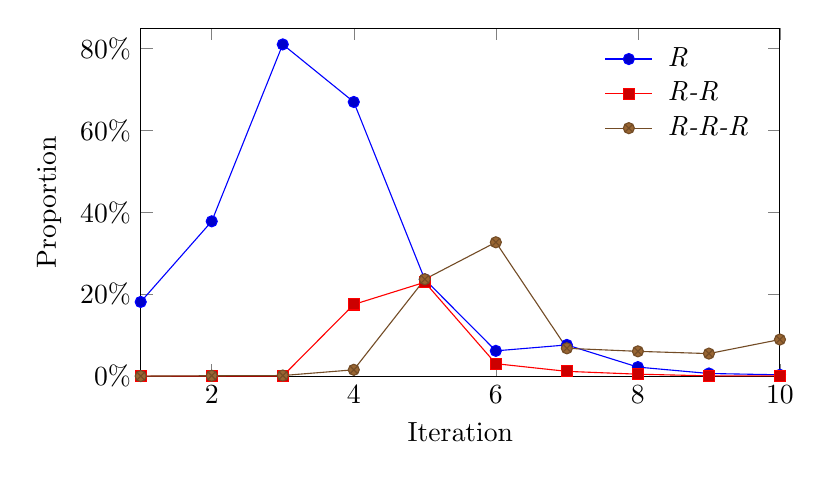
\begin{tikzpicture}
    \begin{axis}[
        width=0.8\linewidth, height=6cm,
        xlabel={Iteration},
        ylabel={Proportion},
        legend pos=north east,
        legend cell align={left},
        ymin=0, ymax=85,
        xmin=1, xmax=10,
        yticklabel={\pgfmathprintnumber{\tick}\%},
        legend style={
            fill=none,
            column sep=1ex,  % Space between columns
            row sep=0.5ex,   % Space between rows
            draw=none, % Remove the black border
            nodes={inner sep=1pt}, % Adjust spacing inside legend entries
        }
    ]
    \pgfplotstableread{
        Iteration  R  R-R  R-R-R
        1  18.12  0.00  0.00 
        2  37.82  0.00  0.09 
        3  81.05  0.01  0.14 
        4  66.98  17.51  1.54 
        5  23.62  22.93  23.67 
        6  6.17  3.03  32.70 
        7  7.62  1.16  6.79 
        8  2.20  0.47  6.05 
        9  0.64  0.06  5.50 
        10  0.32  0.04  8.94 
    }\datatable
    \addplot table[x=Iteration, y=R] from \datatable;
    \addplot table[x=Iteration, y=R-R] from \datatable;
    \addplot table[x=Iteration, y=R-R-R] from \datatable;
    \legend{\textit{R}, \textit{R-R}, \textit{R-R-R}}
    \end{axis}
\end{tikzpicture}
\caption{Distribution of options \textit{R}, \textit{R-R}, and \textit{R-R-R} at the beginning of learning \textit{ms pacman}.}
\label{fig:option-Rs-changing-in-pacman}
\end{figure}


\subsection{Options in the search tree}
\label{appendix:options-in-search}

In this experiment section, we present the detailed statistics in all 26 Atari games conducted for the behavior analysis in Section \ref{sec:behavior-analysis-in-search}.
Specifically, we provide the detailed proportions of options inside the search in Table \ref{tab:option-in-tree-op3-op6}, and the detailed tree depths in Table \ref{tab:tree-depth-op1-op3-op6}.
In Table \ref{tab:option-in-tree-op3-op6}, the columns ``\% Env.'' and ``\% MCTS'' represent the proportions of options applied to the environments and the options suggested by the MCTS process.
Note that due to softmax selection, the options suggested by the tree, ``\% MCTS'', are not always applied, resulting in a lower ``\% Env.''.
Nevertheless, if the suggested options have higher visit counts, they are more likely to be applied, such as in \textit{crazy climber}, \textit{freeway}, and \textit{kung fu master}, where options are well-trained for specific purposes, like climbing, crossing the road, and attacking with an uppercut, respectively, and therefore have higher probabilities of application.
Also, the columns ``\% in Tree'' and ``\% in Sim.'' represent the proportions of the search tree that contains at least one option (in its 50 simulations) and the proportions of simulations whose selection path contains an option.
\revision{In Table \ref{tab:tree-depth-op1-op3-op6}, the columns ``Avg'' and ``Max'' represent the average and the maximum search tree depths; the columns ``$P_{25}$'', ``$P_{50}$'', and ``$P_{75}$'' represent the 25th, 50th, and 75th percentiles.
Based on the $P_{50}$ and $P_{75}$ depths, we observe that the search is not deep in most cases, implying that the models learn to perform deep searches only in certain states.}

\begin{table}[h!]
    \caption{Proportions of options in search tree for $\ell_3$ and $\ell_6$ in 26 Atari games.}
    \centering
    \small
    \resizebox{\textwidth}{!}{
    \begin{tabular}{l|rrrr|rrrr}
        \toprule
        \multirow{2}{*}{Game} & \multicolumn{4}{c|}{$\ell_3$} & \multicolumn{4}{c}{$\ell_6$} \\
        & \% Env. & \% MCTS & \% in Tree & \% in Sim. & \% Env. & \% MCTS & \% in Tree & \% in Sim. \\
        \midrule
        alien & 32.34\% & 52.05\% & 99.81\% & 35.85\% & 30.72\% & 54.92\% & 96.80\% & 24.13\% \\
        amidar & 34.49\% & 52.26\% & 90.68\% & 31.95\% & 32.38\% & 48.54\% & 90.17\% & 26.82\% \\
        assault & 21.16\% & 33.99\% & 82.15\% & 11.93\% & 21.29\% & 35.45\% & 90.45\% & 11.95\% \\
        asterix & 7.18\% & 15.02\% & 63.52\% & 7.11\% & 7.32\% & 17.19\% & 51.50\% & 4.99\% \\
        bank heist & 58.07\% & 74.56\% & 99.45\% & 33.10\% & 51.83\% & 73.85\% & 97.71\% & 22.65\% \\
        battle zone & 11.11\% & 30.41\% & 83.91\% & 14.91\% & 8.46\% & 26.67\% & 80.12\% & 9.89\% \\
        boxing & 60.47\% & 77.80\% & 99.09\% & 40.69\% & 51.54\% & 73.50\% & 98.70\% & 33.12\% \\
        breakout & 21.00\% & 43.77\% & 90.74\% & 15.52\% & 18.79\% & 49.61\% & 90.37\% & 13.65\% \\
        chopper command & 23.92\% & 41.11\% & 88.99\% & 21.96\% & 17.25\% & 33.43\% & 90.46\% & 15.90\% \\
        crazy climber & 49.07\% & 67.94\% & 98.69\% & 39.96\% & 39.31\% & 59.56\% & 98.53\% & 37.09\% \\
        demon attack & 23.30\% & 36.21\% & 93.16\% & 16.04\% & 17.36\% & 29.88\% & 82.75\% & 11.65\% \\
        freeway & 60.80\% & 86.08\% & 99.11\% & 43.83\% & 54.62\% & 74.97\% & 98.75\% & 38.75\% \\
        frostbite & 41.90\% & 65.81\% & 97.58\% & 41.18\% & 33.20\% & 61.49\% & 96.33\% & 30.52\% \\
        gopher & 48.56\% & 63.83\% & 99.17\% & 25.33\% & 43.88\% & 65.21\% & 99.37\% & 20.31\% \\
        hero & 18.28\% & 39.68\% & 74.43\% & 20.07\% & 10.42\% & 26.64\% & 62.88\% & 11.60\% \\
        jamesbond & 48.66\% & 67.76\% & 99.16\% & 39.10\% & 33.92\% & 52.62\% & 97.87\% & 27.33\% \\
        kangaroo & 70.16\% & 86.86\% & 99.64\% & 55.49\% & 60.00\% & 78.64\% & 99.69\% & 44.32\% \\
        krull & 32.28\% & 54.00\% & 99.04\% & 27.34\% & 39.69\% & 69.86\% & 99.79\% & 28.64\% \\
        kung fu master & 61.52\% & 80.42\% & 99.62\% & 41.06\% & 46.91\% & 68.90\% & 99.80\% & 30.53\% \\
        ms pacman & 34.99\% & 56.34\% & 96.90\% & 30.82\% & 22.87\% & 39.34\% & 95.10\% & 21.84\% \\
        pong & 75.43\% & 86.98\% & 99.46\% & 54.27\% & 63.18\% & 77.40\% & 99.48\% & 43.50\% \\
        private eye & 6.40\% & 27.84\% & 67.01\% & 7.61\% & 2.96\% & 14.88\% & 44.25\% & 5.44\% \\
        qbert & 49.96\% & 72.41\% & 99.16\% & 38.83\% & 37.21\% & 59.20\% & 93.98\% & 29.35\% \\
        road runner & 14.05\% & 28.43\% & 62.98\% & 12.36\% & 3.81\% & 8.70\% & 33.76\% & 3.99\% \\
        seaquest & 25.12\% & 44.43\% & 95.88\% & 16.88\% & 17.59\% & 31.77\% & 92.72\% & 13.66\% \\
        up n down & 47.94\% & 66.05\% & 97.74\% & 29.12\% & 28.35\% & 44.52\% & 93.03\% & 17.53\% \\
        \midrule
        Average & 37.62\% & 55.85\% & 91.43\% & 28.94\% & 30.57\% & 49.11\% & 87.48\% & 22.28\% \\
        \bottomrule
    \end{tabular}
    }
    \label{tab:option-in-tree-op3-op6}
\end{table}

\begin{table}[h]
    \caption{Tree depths for $\ell_1$, $\ell_3$, and $\ell_6$ in 26 Atari games.}
    \centering
    \small
    \resizebox{\textwidth}{!}{
    {\setlength{\tabcolsep}{0.25em}
    \begin{tabular}{l|rrrrr|rrrrr|rrrrr}
        \toprule
        \multirow{2}{*}{Game} & \multicolumn{5}{c|}{$\ell_1$} & \multicolumn{5}{c|}{$\ell_3$} & \multicolumn{5}{c}{$\ell_6$} \\
         & Avg & \revision{$P_{25}$} & \revision{$P_{50}$} & \revision{$P_{75}$} & Max & Avg & \revision{$P_{25}$} & \revision{$P_{50}$} & \revision{$P_{75}$} & Max & Avg & \revision{$P_{25}$} & \revision{$P_{50}$} & \revision{$P_{75}$} & Max \\
        \midrule
        alien & 17.99 & \revision{10} & \revision{14} & \revision{26} & 50 & 24.19 & \revision{13} & \revision{20} & \revision{31} & 123 & 29.61 & \revision{13} & \revision{22} & \revision{42} & 259 \\
        amidar & 13.17 & \revision{8} & \revision{11} & \revision{16} & 49 & 22.62 & \revision{10} & \revision{20} & \revision{32} & 135 & 31.43 & \revision{10} & \revision{22} & \revision{43} & 276 \\
        assault & 9.86 & \revision{7} & \revision{9} & \revision{12} & 45 & 8.81 & \revision{6} & \revision{8} & \revision{11} & 78 & 9.30 & \revision{7} & \revision{9} & \revision{11} & 127 \\
        asterix & 10.39 & \revision{6} & \revision{7} & \revision{11} & 49 & 7.83 & \revision{5} & \revision{7} & \revision{9} & 100 & 7.15 & \revision{5} & \revision{6} & \revision{8} & 102 \\
        bank heist & 13.77 & \revision{12} & \revision{13} & \revision{15} & 49 & 17.10 & \revision{14} & \revision{17} & \revision{20} & 88 & 16.22 & \revision{12} & \revision{15} & \revision{19} & 114 \\
        battle zone & 16.70 & \revision{8} & \revision{13} & \revision{24} & 49 & 11.36 & \revision{6} & \revision{9} & \revision{13} & 105 & 10.93 & \revision{6} & \revision{8} & \revision{12} & 144 \\
        boxing & 15.13 & \revision{11} & \revision{15} & \revision{18} & 46 & 27.96 & \revision{15} & \revision{23} & \revision{37} & 107 & 38.43 & \revision{14} & \revision{23} & \revision{54} & 187 \\
        breakout & 11.86 & \revision{7} & \revision{11} & \revision{15} & 43 & 10.64 & \revision{7} & \revision{9} & \revision{13} & 90 & 9.49 & \revision{7} & \revision{9} & \revision{11} & 83 \\
        chopper command & 12.03 & \revision{7} & \revision{10} & \revision{15} & 49 & 15.58 & \revision{8} & \revision{12} & \revision{20} & 141 & 13.13 & \revision{7} & \revision{10} & \revision{16} & 228 \\
        crazy climber & 17.90 & \revision{11} & \revision{17} & \revision{24} & 50 & 36.12 & \revision{15} & \revision{34} & \revision{51} & 147 & 61.50 & \revision{15} & \revision{51} & \revision{101} & 288 \\
        demon attack & 9.52 & \revision{6} & \revision{8} & \revision{11} & 49 & 11.17 & \revision{7} & \revision{10} & \revision{13} & 135 & 9.88 & \revision{6} & \revision{8} & \revision{12} & 222 \\
        freeway & 15.03 & \revision{10} & \revision{14} & \revision{19} & 48 & 27.56 & \revision{15} & \revision{21} & \revision{35} & 135 & 44.50 & \revision{17} & \revision{34} & \revision{60} & 210 \\
        frostbite & 23.28 & \revision{12} & \revision{19} & \revision{34} & 50 & 31.05 & \revision{15} & \revision{25} & \revision{41} & 147 & 44.56 & \revision{12} & \revision{21} & \revision{55} & 294 \\
        gopher & 12.98 & \revision{10} & \revision{13} & \revision{15} & 46 & 17.01 & \revision{12} & \revision{16} & \revision{21} & 114 & 15.16 & \revision{11} & \revision{14} & \revision{18} & 145 \\
        hero & 22.30 & \revision{10} & \revision{19} & \revision{33} & 50 & 17.06 & \revision{6} & \revision{10} & \revision{21} & 147 & 14.80 & \revision{5} & \revision{7} & \revision{13} & 276 \\
        jamesbond & 20.28 & \revision{10} & \revision{17} & \revision{29} & 50 & 25.91 & \revision{14} & \revision{25} & \revision{35} & 138 & 28.77 & \revision{13} & \revision{24} & \revision{41} & 246 \\
        kangaroo & 17.89 & \revision{11} & \revision{16} & \revision{23} & 49 & 39.29 & \revision{25} & \revision{39} & \revision{52} & 150 & 46.69 & \revision{24} & \revision{40} & \revision{62} & 223 \\
        krull & 10.29 & \revision{7} & \revision{9} & \revision{12} & 48 & 15.24 & \revision{9} & \revision{13} & \revision{19} & 64 & 21.65 & \revision{12} & \revision{17} & \revision{22} & 204 \\
        kung fu master & 15.83 & \revision{12} & \revision{15} & \revision{19} & 49 & 26.10 & \revision{19} & \revision{26} & \revision{32} & 84 & 27.27 & \revision{16} & \revision{26} & \revision{36} & 138 \\
        ms pacman & 14.87 & \revision{8} & \revision{12} & \revision{20} & 49 & 21.51 & \revision{10} & \revision{17} & \revision{30} & 135 & 23.58 & \revision{9} & \revision{15} & \revision{31} & 169 \\
        pong & 23.21 & \revision{15} & \revision{23} & \revision{31} & 50 & 50.28 & \revision{28} & \revision{48} & \revision{67} & 144 & 67.51 & \revision{19} & \revision{60} & \revision{102} & 264 \\
        private eye & 10.61 & \revision{4} & \revision{6} & \revision{16} & 50 & 8.22 & \revision{5} & \revision{7} & \revision{10} & 129 & 6.22 & \revision{2} & \revision{5} & \revision{8} & 168 \\
        qbert & 13.09 & \revision{7} & \revision{11} & \revision{17} & 48 & 26.83 & \revision{15} & \revision{25} & \revision{36} & 138 & 38.31 & \revision{13} & \revision{30} & \revision{59} & 228 \\
        road runner & 8.17 & \revision{4} & \revision{5} & \revision{10} & 49 & 10.14 & \revision{5} & \revision{7} & \revision{10} & 120 & 6.61 & \revision{4} & \revision{5} & \revision{6} & 139 \\
        seaquest & 10.94 & \revision{8} & \revision{10} & \revision{12} & 49 & 12.34 & \revision{8} & \revision{10} & \revision{13} & 114 & 11.43 & \revision{7} & \revision{9} & \revision{13} & 115 \\
        up n down & 10.40 & \revision{7} & \revision{10} & \revision{13} & 49 & 17.42 & \revision{11} & \revision{16} & \revision{22} & 150 & 13.91 & \revision{9} & \revision{13} & \revision{18} & 288 \\
        \midrule
        Average & 14.52 & \revision{8.77} & \revision{12.58} & \revision{18.85} & 48.54 & 20.74 & \revision{11.65} & \revision{18.23} & \revision{26.69} & 121.46 & 24.92 & \revision{10.58} & \revision{19.35} & \revision{33.58} & 197.58 \\
        \bottomrule
    \end{tabular}
    }
    }
    \label{tab:tree-depth-op1-op3-op6}
\end{table}

\clearpage

\subsection{Prediction accuracy of options}

In this experiment, we check how the options suggested by the MCTS process predict future actions.
For example, if an option \textit{R-R-R} is suggested by the search at time $t$, we calculate the prediction accuracy using the recorded actions $a_t$, $a_{t+1}$, and $a_{t+2}$.
The results for both $\ell_3$ and $\ell_6$ are shown in Table \ref{tab:option-prediction-op3-op6}.
% We notice that the prediction accuracy is correlated with the probability of applying suggested options to the environment (analyzed in Table \ref{tab:option-in-tree-op3} and Table \ref{tab:option-in-tree-op6}).
As expected, the prediction accuracy decreases as the number of steps increases.
Interestingly, the accuracy of the 1-step is higher than that of the 0-step.
We assume this phenomenon is caused by softmax selection for options with repeated primitive actions.
For example, the agent may apply \textit{U} than the suggested options \textit{R-R-R}.
When this happens, at step $t+1$, there is likely a much higher probability of acting \textit{R} again to prompt the original decision.
On the other hand, the prediction accuracy of $\ell_6$ is generally lower than those of $\ell_3$ at the same step number.
It is hypothesized that increasing the maximum option length also increases the difficulty of training prediction and dynamics networks, thereby lowering the accuracy.
To summarize, this observation verifies that the learned options closely correspond to the probabilities of choosing primitive actions.

\begin{table}
    \caption{Prediction accuracy between options and environmental actions for $\ell_3$ and $\ell_6$ in 26 Atari games.}
    \centering
    \small
    \resizebox{\textwidth}{!}{
    \begin{tabular}{l|rrr|rrrrrr}
        \toprule
        \multirow{2}{*}{Game} & \multicolumn{3}{c|}{$\ell_3$} & \multicolumn{6}{c}{$\ell_6$} \\
        & 0-step & 1-step & 2-step & 0-step & 1-step & 2-step & 3-step & 4-step & 5-step \\
        \midrule
        alien & 73.43\% & 81.24\% & 66.76\% & 68.84\% & 75.00\% & 61.55\% & 56.89\% & 53.50\% & 51.49\% \\
        amidar & 75.55\% & 81.32\% & 71.78\% & 78.02\% & 82.90\% & 62.28\% & 55.19\% & 50.08\% & 48.32\% \\
        assault & 76.61\% & 83.70\% & 35.49\% & 76.55\% & 83.98\% & 37.41\% & 11.58\% & 3.94\% & 1.48\% \\
        asterix & 64.41\% & 71.68\% & 29.46\% & 63.54\% & 69.28\% & 13.08\% & 7.10\% & 4.16\% & 2.59\% \\
        bank heist & 91.84\% & 93.82\% & 72.82\% & 90.59\% & 91.42\% & 55.11\% & 35.85\% & 23.09\% & 15.64\% \\
        battle zone & 59.31\% & 68.10\% & 35.97\% & 53.03\% & 62.06\% & 33.77\% & 22.97\% & 18.79\% & 16.86\% \\
        boxing & 87.66\% & 92.72\% & 76.38\% & 85.41\% & 89.93\% & 64.36\% & 51.47\% & 45.70\% & 41.32\% \\
        breakout & 65.61\% & 72.96\% & 33.90\% & 58.44\% & 65.56\% & 19.29\% & 5.35\% & 2.77\% & 1.80\% \\
        chopper command & 71.11\% & 76.93\% & 51.90\% & 69.16\% & 74.82\% & 33.97\% & 23.98\% & 19.02\% & 13.41\% \\
        crazy climber & 84.24\% & 91.40\% & 77.09\% & 83.95\% & 89.90\% & 67.90\% & 57.60\% & 53.24\% & 50.56\% \\
        demon attack & 76.62\% & 84.59\% & 53.52\% & 73.07\% & 81.17\% & 35.98\% & 19.92\% & 12.17\% & 8.97\% \\
        freeway & 76.15\% & 85.47\% & 83.13\% & 80.20\% & 88.91\% & 80.89\% & 77.34\% & 75.54\% & 74.57\% \\
        frostbite & 73.53\% & 80.95\% & 75.86\% & 68.05\% & 75.05\% & 67.44\% & 62.74\% & 59.82\% & 57.79\% \\
        gopher & 85.18\% & 90.50\% & 71.23\% & 80.08\% & 86.74\% & 41.73\% & 28.23\% & 20.99\% & 17.57\% \\
        hero & 60.77\% & 69.45\% & 56.73\% & 60.65\% & 67.48\% & 47.38\% & 41.79\% & 39.61\% & 37.74\% \\
        jamesbond & 80.04\% & 85.72\% & 70.20\% & 76.12\% & 82.04\% & 63.76\% & 55.58\% & 52.27\% & 49.35\% \\
        kangaroo & 88.71\% & 91.89\% & 84.32\% & 86.98\% & 90.48\% & 76.48\% & 68.02\% & 61.90\% & 59.13\% \\
        krull & 73.75\% & 81.45\% & 49.56\% & 75.78\% & 82.41\% & 57.58\% & 35.83\% & 24.81\% & 19.37\% \\
        kung fu master & 85.54\% & 90.36\% & 77.14\% & 84.72\% & 89.95\% & 58.19\% & 47.24\% & 39.70\% & 36.20\% \\
        ms pacman & 71.76\% & 78.05\% & 68.81\% & 70.02\% & 79.43\% & 49.92\% & 40.89\% & 37.39\% & 36.39\% \\
        pong & 90.04\% & 94.63\% & 89.50\% & 86.81\% & 92.52\% & 80.49\% & 74.85\% & 69.73\% & 66.69\% \\
        private eye & 53.14\% & 61.30\% & 18.11\% & 47.93\% & 61.86\% & 21.19\% & 12.62\% & 9.67\% & 7.98\% \\
        qbert & 76.17\% & 82.71\% & 79.03\% & 75.21\% & 83.02\% & 72.12\% & 63.94\% & 59.87\% & 57.88\% \\
        road runner & 68.14\% & 71.35\% & 39.60\% & 65.75\% & 73.07\% & 34.80\% & 26.09\% & 21.45\% & 19.21\% \\
        seaquest & 76.62\% & 82.36\% & 37.48\% & 74.19\% & 80.98\% & 35.47\% & 21.45\% & 15.91\% & 12.74\% \\
        up n down & 80.72\% & 88.11\% & 77.24\% & 77.96\% & 87.10\% & 56.07\% & 43.43\% & 34.44\% & 30.06\% \\
        \midrule
        Average & 75.64\% & 82.03\% & 60.89\% & 73.50\% & 80.27\% & 51.09\% & 40.31\% & 34.98\% & 32.12\% \\
        \bottomrule
    \end{tabular}
    }
    \label{tab:option-prediction-op3-op6}
\end{table}

\clearpage


\subsection{Top frequently used options}
\label{appendix:topk-analysis}

Finally, we investigate the distribution of frequently used options for each game.
The accumulated usages are summarized in Table \ref{tab:option-topk-usage-op3-op6}.
Additionally, we extract the top 3 frequently used options for both $\ell_3$ and $\ell_6$ in Table \ref{tab:option-top3-op3} and Table \ref{tab:option-top3-op6}.
% Note that the columns ``\# \{$a$\}'', ``\# \{$o$\}'' represent the numbers of types of actions and types of discovered options.
% , and ``Top $k$'' , and the accumulated usage of the top-$\ceil{k|\#\{$o$\}|}$ frequently used options.
Generally speaking, the distribution of frequently used options is similar between $\ell_3$ and $\ell_6$, where the distribution is highly unbalanced, with the top 25\% options accounting for over 95\% of the usage.
The most extreme case occurs in \textit{freeway}, where the top 1\% (options with repeated \textit{U}) takes a proportion of more than 80\%.
% On the other hand, the top 1\% options only account for 19.11\% in \textit{crazy climber}, relatively lower than in other games.
% We observe that it is due to the requirement of combining \textit{U} and \textit{D} for climbing and \textit{L} and \textit{R} for choosing direction.
On the other hand, for \textit{crazy climber} and \textit{ms pacman}, the top 1\% usages have both been significantly increased from $\ell_3$ to $\ell_6$.
However, the increase in usage does not correlate to the performance, as $\ell_6$ outperforms $\ell_3$ in \textit{crazy climber} but underperforms in \textit{ms pacman}, as shown in Table \ref{tab:Atari26-score}.
Notably, we observe that from $\ell_3$ to $\ell_6$, the numbers of discovered options only increase by a factor of 2.43 on average, implying that there are not so many options practical for the planning.
This analysis demonstrates that a small proportion of frequently used options play important roles in gameplay, and the number of discovered options will not grow excessively when relaxing the limitation of maximum option length.
% 5d: some more about top 1%

\begin{table}[h!]
    \caption{Accumulated usages of the frequently used options for $\ell_3$ and $\ell_6$ in 26 Atari games.}
    \centering
    \small
    \resizebox{\textwidth}{!}{
    \begin{tabular}{l|rrrr|rrrr}
        \toprule
        \multirow{2}{*}{Game} & \multicolumn{4}{c|}{$\ell_3$} & \multicolumn{4}{c}{$\ell_6$} \\
        & Top 1\% & Top 5\% & Top 10\% & Top 25\% & Top 1\% & Top 5\% & Top 10\% & Top 25\% \\
        \midrule
        alien & 21.67\% & 74.01\% & 89.35\% & 98.64\% & 53.56\% & 81.47\% & 90.76\% & 98.15\% \\
        amidar & 41.82\% & 91.33\% & 98.26\% & 99.50\% & 49.67\% & 83.14\% & 94.95\% & 99.23\% \\
        assault & 29.76\% & 70.26\% & 85.88\% & 97.12\% & 45.96\% & 81.53\% & 91.81\% & 98.31\% \\
        asterix & 30.27\% & 75.00\% & 90.57\% & 97.38\% & 36.46\% & 77.98\% & 88.22\% & 97.86\% \\
        bank heist & 22.46\% & 50.28\% & 71.80\% & 96.60\% & 20.68\% & 54.44\% & 70.90\% & 90.26\% \\
        battle zone & 31.80\% & 74.53\% & 95.23\% & 99.31\% & 41.56\% & 78.69\% & 91.88\% & 98.58\% \\
        boxing & 39.55\% & 59.41\% & 71.47\% & 89.90\% & 29.40\% & 59.22\% & 73.56\% & 90.43\% \\
        breakout & 23.33\% & 61.10\% & 79.71\% & 95.22\% & 39.69\% & 75.29\% & 88.13\% & 97.98\% \\
        chopper command & 40.51\% & 90.41\% & 96.61\% & 99.33\% & 35.91\% & 75.72\% & 91.05\% & 99.05\% \\
        crazy climber & 18.00\% & 52.19\% & 73.53\% & 95.66\% & 52.62\% & 82.73\% & 91.65\% & 98.26\% \\
        demon attack & 36.88\% & 81.62\% & 91.80\% & 97.69\% & 46.19\% & 82.89\% & 92.90\% & 98.65\% \\
        freeway & 87.63\% & 91.25\% & 93.94\% & 97.71\% & 81.13\% & 89.75\% & 94.46\% & 98.51\% \\
        frostbite & 58.73\% & 90.74\% & 96.43\% & 99.21\% & 62.58\% & 86.18\% & 93.24\% & 98.26\% \\
        gopher & 58.17\% & 77.73\% & 86.00\% & 96.81\% & 46.93\% & 83.74\% & 92.58\% & 98.51\% \\
        hero & 57.14\% & 91.52\% & 96.54\% & 99.17\% & 52.72\% & 83.91\% & 91.80\% & 97.92\% \\
        jamesbond & 51.74\% & 85.34\% & 93.23\% & 98.43\% & 55.25\% & 84.53\% & 93.46\% & 98.36\% \\
        kangaroo & 43.29\% & 71.76\% & 81.93\% & 94.30\% & 46.48\% & 74.34\% & 85.05\% & 95.85\% \\
        krull & 23.50\% & 56.37\% & 74.32\% & 93.80\% & 21.42\% & 54.80\% & 73.48\% & 92.43\% \\
        kung fu master & 48.52\% & 79.10\% & 89.64\% & 97.27\% & 46.32\% & 75.97\% & 86.49\% & 96.42\% \\
        ms pacman & 28.04\% & 88.11\% & 96.09\% & 99.22\% & 41.82\% & 75.41\% & 90.17\% & 98.02\% \\
        pong & 59.22\% & 80.07\% & 87.07\% & 95.88\% & 49.13\% & 75.00\% & 86.40\% & 96.14\% \\
        private eye & 37.06\% & 68.97\% & 84.19\% & 97.25\% & 33.63\% & 69.21\% & 81.91\% & 94.19\% \\
        qbert & 53.07\% & 94.42\% & 97.80\% & 99.69\% & 67.30\% & 91.71\% & 96.82\% & 99.30\% \\
        road runner & 28.77\% & 80.77\% & 90.97\% & 98.11\% & 42.47\% & 78.51\% & 89.48\% & 97.43\% \\
        seaquest & 29.84\% & 67.32\% & 80.34\% & 94.60\% & 36.79\% & 73.06\% & 86.27\% & 96.69\% \\
        up n down & 62.27\% & 85.91\% & 94.45\% & 98.97\% & 53.55\% & 86.24\% & 94.25\% & 99.14\% \\
        \midrule
        Average & 40.89\% & 76.52\% & 87.97\% & 97.18\% & 45.74\% & 77.52\% & 88.53\% & 97.07\% \\
\bottomrule
    \end{tabular}
    }
    \label{tab:option-topk-usage-op3-op6}
\end{table}

\begin{table}[h!]
    \caption{The top 3 frequently used options with their total share for $\ell_3$ in 26 Atari games.}
    \centering
    \small
    \begin{tabular}{l|ccc|r}
        \toprule
        Game & Top 1 & Top 2 & Top 3 & \% \\
        \midrule
        alien & UR-UR-UR & LF-LF-LF & UL-UL-UL & 10.01\% \\
        amidar & LF-LF-LF & R-R-R & DF-DF-DF & 18.07\% \\
        assault & R-R & L-L & R-R-R & 9.07\% \\
        asterix & U-U-U & D-D & UL-UL & 2.79\% \\
        bank heist & L-R-L & L-UR-L & DL-UR-DL & 16.79\% \\
        battle zone & DF-DF-DF & DRF-DRF-DRF & LF-LF-LF & 3.53\% \\
        boxing & R-R-R & DR-DR-DR & DRF-DRF-DRF & 23.92\% \\
        breakout & N-N-N & N-N & L-L-L & 10.52\% \\
        chopper command & DF-DF-DF & UF-UF-UF & ULF-ULF-ULF & 9.69\% \\
        crazy climber & D-D-U & U-U-U & U-U-D & 12.16\% \\
        demon attack & R-R-R & L-L-L & LF-LF-LF & 10.77\% \\
        freeway & U-U-U & N-N-N & U-U & 57.12\% \\
        frostbite & D-D-D & UR-UR-UR & DR-DR-DR & 24.61\% \\
        gopher & L-L-L & R-R-R & RF-RF-RF & 26.55\% \\
        hero & R-R-R & DLF-DLF-DLF & LF-LF-LF & 8.11\% \\
        jamesbond & UR-UR-UR & L-DLF-L & L-L-L & 21.31\% \\
        kangaroo & D-D-D & F-F-F & LF-LF-LF & 30.37\% \\
        krull & DL-DL-DL & UR-UR-UR & DL-DL & 10.17\% \\
        kung fu master & DR-DR-DR & DLF-DLF-DLF & ULF-ULF-ULF & 20.89\% \\
        ms pacman & UL-UL-UL & DL-DL-DL & UR-UR-UR & 14.52\% \\
        pong & LF-LF-LF & F-F-F & N-N-N & 48.94\% \\
        private eye & URF-URF & L-L-L & L-L & 2.37\% \\
        qbert & D-D-D & R-R-R & L-L-L & 36.60\% \\
        road runner & DLF-DLF-DLF & UL-UL-UL & DL-DL-DL & 5.82\% \\
        seaquest & DF-DF-DF & DLF-DLF-DLF & DLF-DLF & 6.12\% \\
        up n down & U-U-U & UF-UF-UF & DF-DF-DF & 34.05\% \\
        \bottomrule
    \end{tabular}
    \label{tab:option-top3-op3}
\end{table}

\begin{table}[h!]
    \caption{The top 3 frequently used options with their total share for $\ell_6$ in 26 Atari games.}
    \centering
    \small
    \resizebox{\textwidth}{!}{
    \begin{tabular}{l|ccc|r}
        \toprule
        Game & Top 1 & Top 2 & Top 3 & \% \\
        \midrule
        alien & DR-DR-DR-DR-DR-DR & URF-URF-URF-URF-URF-URF & LF-LF-LF-LF-LF-LF & 13.52\% \\
        amidar & LF-LF-LF-LF-LF-LF & UF-UF-UF-UF-UF-UF & RF-RF-RF-RF-RF-RF & 13.30\% \\
        assault & R-R & L-L & U-L-L & 8.35\% \\
        asterix & UL-UL & UR-UR & D-D & 3.49\% \\
        bank heist & DR-L & UR-L & R-DL & 6.77\% \\
        battle zone & DF-DF-DF-DF-DF-DF & UL-UL-UL-UL-UL-UL & U-U & 2.43\% \\
        boxing & DR-DR-DR-DR-DR-DR & DR-DR & N-N-N-N-N-N & 9.83\% \\
        breakout & F-F & N-N & L-L & 9.75\% \\
        chopper command & UF-UF & DF-DF & DLF-DLF-DLF-DLF-DLF-DLF & 5.29\% \\
        crazy climber & U-U-DL-DL-DL-U & UL-UL-DR-DL-DL-UL & U-U-DL-DL-DR-U & 14.20\% \\
        demon attack & RF-RF & L-L & LF-LF & 6.60\% \\
        freeway & U-U-U-U-U-U & U-U & D-U-U-U-U-U & 45.91\% \\
        frostbite & F-F-F-F-F-F & DF-DF-DF-DF-DF-DF & DRF-DRF-DRF-DRF-DRF-DRF & 14.63\% \\
        gopher & L-L & R-R & R-R-R-R-R-R & 11.25\% \\
        hero & DLF-DLF-DLF-DLF-DLF-DLF & RF-RF-RF-RF-RF-RF & DRF-DRF-DRF-DRF-DRF-DRF & 3.65\% \\
        jamesbond & DL-DL-DL-DL-DL-DL & LF-LF-LF-LF-LF-LF & UR-UR-UR-UR-UR-UR & 11.66\% \\
        kangaroo & R-R-R-R-R-R & L-L-L-L-L-L & DL-DL-DL-DL-DL-DL & 17.11\% \\
        krull & UR-UR-UR-UR-UR-UR & DL-DL & L-L-L-L-L-L & 4.40\% \\
        kung fu master & DR-DR-DLF-DR-DR-DR & L-L-L-L-L-L & URF-URF-URF-URF-URF-URF & 7.57\% \\
        ms pacman & UL-UL-UL-UL-UL-UL & UL-UL & DR-DR-DR-DR-DR-DR & 9.56\% \\
        pong & RF-RF-RF-RF-RF-RF & R-R-R-R-R-R & LF-LF-LF-LF-LF-LF & 24.58\% \\
        private eye & URF-URF & ULF-ULF & DF-DF-DF-DF-DF-DF & 0.78\% \\
        qbert & F-F-F-F-F-F & R-R-R-R-R-R & U-U-U-U-U-U & 21.94\% \\
        road runner & ULF-ULF-ULF-ULF-ULF-ULF & L-L & L-L-L-L-L-L & 1.62\% \\
        seaquest & DLF-DLF & DRF-DRF & DLF-DLF-DLF-DLF-DLF-DLF & 3.30\% \\
        up n down & U-U-U-U-U-U & DF-DF & U-U & 15.18\% \\
        \bottomrule
    \end{tabular}
    }
    \label{tab:option-top3-op6}
\end{table}



% guei: figure for games

% atari_breakout_mz_2bx64_n50-d161f9-dirty_0919_option_act_op3_1\300-217-424 cf.89
% atari_crazy_climber_mz_2bx64_n50-d161f9-dirty_0919_option_act_op3_1\300-214-126200 cf.39
% atari_freeway_mz_2bx64_n50-d161f9-dirty_0919_option_act_op3_1\300-235-31 cf.13
% atari_hero_mz_2bx64_n50-d161f9-dirty_0919_option_act_op3_1\300-171-20530 cf.3
% atari_kung_fu_master_mz_2bx64_n50-d161f9-dirty_0919_option_act_op3_1\300-217-56400 cf.60
% atari_ms_pacman_mz_2bx64_n50-d161f9-dirty_0919_option_act_op3_1 300-248-6550 cf.95
% atari_pong_mz_2bx64_n50-d161f9-dirty_0919_option_act_op3_1\300-246-7 cf.16
% atari_seaquest_mz_2bx64_n50-d161f9-dirty_0919_option_act_op3_1\300-248-8040 cf.104
% \begin{figure}[h!]
%     \centering
%     \includegraphics[width=1\linewidth]{tmp-selected-atari-games.png}
%     \caption{tmp-selected-atari-games}
%     \label{fig:tmp-selected-atari-games}
% \end{figure}
